\newpage
\section{Требования к системе}
\subsection{Основные правила игры <<Монополия>>}
Для правильного определения требований к разрабатываемой системе необходимо сначала выделить основные правила разрабатываемой игры.

«Монополия» - это экономическая пошаговая стратегия. Главная цель игры – рационально использовать полученный вначале капитал, который выдаётся всем игрокам в равном объёме, и привести к банкротству других участников. Пошаговый игровой процесс разбивается на ходы, каждый игрок ходит по очереди. Игрок перемещается по игровому полю в зависимости от количества очков, выпавшему на кубиках. Если выпал дубль, то игрок повторяет свой ход. В зависимости от клетки, на которую игрок попадает совершаются разнообразные действия.

Помимо перемещения и выполнения действий, приписанных этой клетке игрок вправе:
\begin{spacing}{0.9}
\begin{enumerate}
    \item Участвовать в аукционах недвижимости, которую отказывались покупать другие игроки 
    \item Улучшать свои владения посредством покупки домов для увеличения арендной платы, которая платится другими игроками при попадании на клетку недвижимости
    \item Продавать дома по необходимости
    \item Закладывать участки недвижимости при отсутствии денег
    \item Выкупать свои участки из залога
\end{enumerate}
\end{spacing}

\textbf{Объекты игры}

На игровом поле расположены клетки. В начале игры каждый игрок располагается на начальной клетке «Вперёд». Всего клетки могут быть разных типов:
\begin{spacing}{0.9}
\begin{enumerate}
    \item Улица – поле доступное для покупки, улицы делятся на группы по цвету, завладев одним цветом, игрок вправе купить дом на данной улице. Если игрок попадает на данное поле, и оно не принадлежит никому, то он вправе его купить за указанную стоимость. Если игрок попадает на данном поле, и оно принадлежит другому игроку, то игрок платит арендную плату этому игроку в зависимости от уровня развития данной улицы. Аналогичная логика используется на полях «Коммунальное предприятие» и «Железнодорожная станция». 
    \item Коммунальное предприятие – поле доступное для покупки, арендная плата на нем считается в зависимости от количества выпавших очков
    \item Железнодорожная станция – поле доступное для покупки, арендная плата на нём считается в зависимости от количества купленных полей данного типа у владельца поля.
    \item «Шанс» и «Общественная казна» -  поля, на которых игрок должен выполнить действие, которое случайно выберет игра.
    \item Бесплатная стоянка – поле, на котором ничего не происходит
    \item «Налог» - игрок обязан выплатить определенную сумму налога
\end{enumerate}
\end{spacing}

\textbf{Тюрьма}

Игрок отправляется в Тюрьму, если:
\begin{spacing}{0.9}
\begin{enumerate}
    \item Остановится на поле «Отправляйтесь в Тюрьму» 
    \item Игрок взял карточку «Шанс» или «Общественная казна», на которой написано «Отправляйтесь в Тюрьму»
    \item У игрока выпало одинаковое число очков на обоих кубиках три раза подряд за один ход
\end{enumerate}
\end{spacing}

Ход игрока оканчивается, когда его отправляют в Тюрьму. 

Чтобы выйти из Тюрьмы, игроку необходимо:
\begin{spacing}{0.9}
\begin{enumerate}
    \item Заплатить штраф в размере 50 рублей и продолжить игру
    \item Попытаться выбросить дубль
\end{enumerate}
\end{spacing}

После того, как игрок пропустит три хода, находясь в Тюрьме, он должен выйти из неё и уплатить 50 тыс. рублей, прежде чем сможет переместиться на такое число полей, которое выпало на кубиках. 

Находясь в Тюрьме, игрок может получать арендную плату за недвижимость, если она не заложена. Если игрок не был «отправлен в Тюрьму», а просто остановился на поле «Тюрьма» в ходе игры, то он не платит никакого штрафа.

\textbf{Залог}

Если у игрока не хватает денег, то он вправе заложить определенное поле. Для этого, сначала продаются все дома, расположенные на данной клетке, если такие имеются и затем игроку передаётся половина от стоимости клетки. 

После этого, если другой игрок окажется на данной клетке, то арендная плата взыматься не будет. Однако с других клеток плата взыматься будет.

Для того, чтобы выкупить данную клетку, игроку необходимо внести половину стоимости клетки + 10\%.

\textbf{Покупка домов}

Если игрок купил всю цветовую группу клеток, то он монополизировал данную цветовую группу и вправе строить дома на ней. Однако, если хоть одна клетка из цветовой группы заложена, то игрок теряет данную возможность.

Постройка домов увеличивает арендную плату. На одной клетке можно построить максимум 4 дома

\textbf{Банкротство}

Если игрок должен Банку или другому игроку больше денег, чем может получить по своим активам, то он объявляется банкротом, и выбывает из игры

Если игрок должен Банку, Банк получает все деньги игрока. Затем вся недвижимость обанкротившегося игрока продаётся с аукциона.

Если игрок должен другому игроку, все дома банкрота продаются, полученные средства передаются игроку, обанкротившему его, как и вся недвижимость, включая заложенную.
\subsection{Функциональные требования}
\begin{spacing}{0.9}
\begin{enumerate}
    \item Система игра «Монополия» должна реализовывать основные правила настольной игры 
    \item Система игра «Монополия» должна поддерживать локальный многопользовательский режим
    \item Система игра «Монополия» должна правильно определять победителя партии.
\end{enumerate}
\end{spacing}
\subsection{Нефункциональные требования}
\begin{spacing}{0.9}
\begin{enumerate}
    \item Система игра «Монополия» должна быть написана на языке Python 
    \item Система игра «Монополия» должна поддерживать как реальных игроков, так и ботов
    \item Система игра «Монополия» должна реализовывать текстовый интерфейс
\end{enumerate}
\end{spacing}
\subsection{Диаграмма вариантов использования}
Система представляет собой программу, реализующую игру «Монополия».

Единственным актёром системы является игрок.
\begin{figure}[h!]
    \center{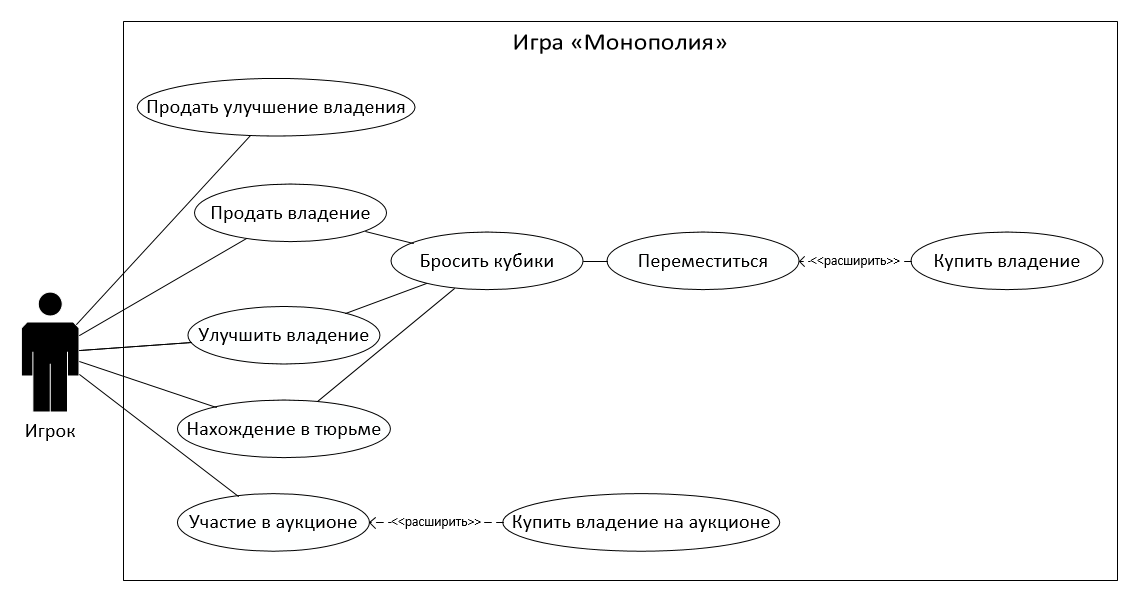
\includegraphics[width=1\linewidth]{use-case.png}}
    \caption{Диаграмма вариантов использования}
\end{figure}

Определим основные варианты использования системы игра «Монополия». Пользователю доступны следующие функции:
\begin{enumerate}
    \item \textit{Продать улучшение владения} – игрок может продать ненужные улучшения его владений во время своего хода для получения дополнительного заработка
    \item \textit{Продать владение} – игрок может продать ранее приобретённые владения
    \item \textit{Улучшить владение} – игрок может улучшить приобретённое владение, если цветовая группа владения находится под контролём его монополии
    \item \textit{Нахождение в тюрьме} – игрок может находиться в тюрьме определённое количество ходов
    \item \textit{Участие в аукционе} – игрок может участвовать в уникальном событии – аукционе
    \item \textit{Бросить кубики} – игрок бросает кубики для определения количества клеток для перемещения
    \item \textit{Переместиться} – игрок перемещается на выпавшее количество очков
    \item \textit{Купить владение} – игрок может купить владение, на которое он попал, если оно не принадлежит никому
\end{enumerate}
\subsection{Спецификация основных вариантов использования}
\newpage
\begin{table}[h!]
\caption{Спецификация прецедента <<Нахождение в тюрьме>>}
\begin{tabular}{|l|}
    \hline
    \textbf{UseCase: Нахождение в тюрьме}\\
    \hline
    \textit{Аннотация:}\ Нахождение игрока в тюрьме\\
    \hline
    Главные актеры: Игрок \\
    \hline
    Второстепенные актеры: Нет \\
    \hline
    Предусловия: Игрок находится в тюрьме \\
    \hline
    Основной поток: \\
        1)Система проверяет количество ходов, проведенных в тюрьме игроком \\
        2)Игроку предлагается купить выход из тюрьмы \\
        3)Игрок выплачивает штраф за выход из тюрьмы \\
        4)Игрок выходит из тюрьмы \\
    \hline
    Постусловия: Игрок вышел из тюрьмы\\
    \hline
    Альтернативные потоки:\\
    2А Игрок отказался покупать выход из тюрьмы\\
    1)Игрок остаётся в тюрьме\\
    1А Игрок слишком долго находится в тюрьме\\
    1)Игрок выплачивает штраф за выход из тюрьмы\\
    2)Игрок выходит из тюрьмы\\
    4А Игрок не в состоянии оплатить штраф за выход из тюрьмы\\
    1)Система предлагает игроку продать владения\\
    2)Игрок продаёт владения\\
    3)Игрок выплачивает штраф за выход из тюрьмы\\
    4)Игрок выходит из тюрьмы\\
    4А 1А Игрок не имеет владений, игрок отказался продавать владения\\
    1)Игрок становится банкротом\\
    2)Все владения игрока продаются на аукционе\\
    \hline
\end{tabular}  
\end{table}
\newpage
\begin{table}[h!]
    \caption{Спецификация прецедента <<Купить владение>>}
    \begin{tabular}{|l|}
        \hline
        \textbf{UseCase: Купить владение}\\
        \hline
        \textit{Аннотация:}\ Нахождение игрока в тюрьме\\
        \hline
        Главные актеры: Игрок \\
        \hline
        Второстепенные актеры: Нет \\
        \hline
        Предусловия: Владение никому не принадлежит и доступно для покупки \\
        \hline
        Основной поток: \\
            1)Система предлагает купить владение \\
            2)Игрок решает купить владение \\
            3)Система проверяет возможность покупки владения игроком \\
            4)Игрок завладевает ячейкой\\
        \hline
        Постусловия: Ход передаётся следующему игроку\\
        \hline
        Альтернативные потоки:\\
        2А Игрок отказывается от покупки, 3А Игроку не хватает денег для покупки\\
        1)Ячейка выставляется на аукционе\\
        2)Все игроки оповещаются о начале аукциона\\
        \hline
    \end{tabular}  
\end{table}
\subsection*{Выводы}
\addcontentsline{toc}{subsection}{Выводы}
В процессе анализа требований был определен основной актер системы, варианты использования системы, сформулированы основные функциональные и нефункциональные требования, предъявляемые к разрабатываемой системе.